\section{Ziel}
In diesem Versuch wird eine Hochvakuumdiode untersucht, um  die Austrittsarbeit der Elektronen bei Wolfram zu bestimmen.
Hierzu werden verschiedene Kennlinien gemessen und der Gültigkeitsbereich des Langmuir-Schottkyschen Raumladungsgesetzes gesucht.
Außerdem wird das Anlaufstromgebiet der Diode untersucht.






\section[Theorie]{Theorie\footnote[1]{Unter Verwendung von \cite{man:v504}.}}

% \subsection{Einleitung}
Grundlage dieses Versuchs ist der glühelektrische Effekt, bei dem durch Erwärmung von Metalloberflächen Elektronen emittiert werden können.
Dabei ist insbesondere die Austrittsarbeit als Materialkonstante von Interesse.
Hierfür ist eine Hochvakuumdiode nötig, damit die Elektronen nicht mit der Luft wechselwirken.



\subsection{Austrittsarbeit und Energieverteilung von Leitungselektronen}
In Metallen sind ionisierte Atome auf einer Kristallgitterstruktur angeordnet.
Die Atome sind dabei von freigesetzten Elektronen eingehüllt, die nicht mehr einem bestimmten Atom zugeordnert werden können.
Daher werden sie auch Leitungselektronen genannt.
In grober Näherung kann für das Gitterpotential das Potentialtopfmodell verwendet werden.
Im Inneren des Metalls gibt es dabei ein positives konstantes Potential, welches allerdings um den Betrag $\xi$ geringer ist als im Außenraum des Metalls, vgl. Abbilung \ref{fig:potentialtopf_metall}.
Auf die Leitungselektronen wirken folglich keine Kräfte und sie können sich frei bewegen.
Deshalb haben Metalle eine sehr gute elektrische Leitfähigkeit.
Zum Verlassen des Metalls muss ein Elektron somit die Austrittsarbeit
\begin{align}
    W = \text{e}_0 \xi
    \label{eq:austrittsarbeit}
\end{align}
aufwenden.

\begin{figure}[H]
    \centering
    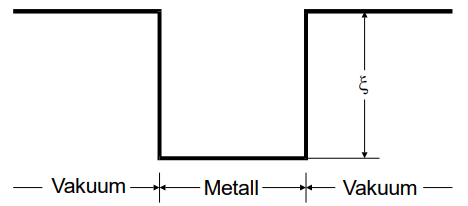
\includegraphics[height = 3 cm]{Abbildungen/potentialtopf_metall.png}
    \caption{Schematische Darstellung des Potentialtopfes eines Metalls \cite[]{man:v504}.}
    \label{fig:potentialtopf_metall}
\end{figure}


\noindent
Um zu überprüfen, ob die innere Energie der Elektronen zum spontanen Verlassen der Oberfläche ausreicht, muss die Quantentheorie betrachtet werden.
Zum einen können die Elektronen nur diskrete Energiewerte annnehmen.
Zum anderen kann ein Zustand mit Energie $E$ aufgrund des Pauli-Verbots von maximal 2 Elektronen mit entgegengesetzten Spin besetzt werden.
Dadurch haben die Elektronen selbst für $T = 0$ eine endliche Energie, 
die sogenannte Fermische Grenzenergie $\zeta$, für die bei Zimmertemperatur $\zeta >> k_\text{B} T$ gilt.
Die Fermi-Diracsche Verteilungsfuktion beschreibt die Wahrscheinlichkeit, dass im thermischen Gleichgewicht ein möglicher Zustand mit der Energie $E$ besetzt ist.
Dadurch, dass selbst beim Schmelzpunkt von Wolfram $E$ groß gegen $k_\text{B} T$ ist, kann die Funktion durch
\begin{align}
    f(E) = \exp\left(\frac{\zeta - E}{k_\text{B} T}\right)
    \label{eq:energieverteilung}
\end{align}
genähert werden.




\subsection{Die Sättigungsstromdichte}